\chapter{Vector spaces}

A vector space over a field \(\mathbb F\) is a non-empty set \(V\) together with two binary operations. It is indicated as a triplet: $(V, +, \cdot)$.

A vector space must satisfy the ten axioms listed below.

{\large$$\forall \vec v, \vec w, \vec u \in V \land \forall a, b \in \mathbb F$$}

\begin{itemize}
\item \textbf{Closure under "+" operation:}
    $\vec v + \vec w \in V$
\item \textbf{Closure under "·" operation:}
    $a \cdot \vec v \in V$
\item \textbf{Associativity of vector addition:} $\vec{u} + (\vec{v} + \vec{w}) = (\vec{u} + \vec{v}) + \vec{w}$
\item \textbf{Commutativity of vector addition:} $\vec{u} + \vec{v} = \vec{v} + \vec{u}$
\item \textbf{Identity element of vector addition:} There exists an element $\vec{0} \in V$, called the zero vector, such that $\vec{v} + \vec{0} = \vec{v}$.
\item \textbf{Inverse elements of vector addition:} $\exists -\vec{v} \in V$ called the additive inverse of $\vec{v}$, such that $\vec{v} + (-\vec{v}) = \vec{0} \in V$.
\item \textbf{Compatibility of scalar multiplication with field multiplication:} $a(b\vec{v}) = (ab)\vec{v}$.
\item \textbf{Identity element of scalar multiplication:} $1\vec{v} = \vec{v}$ where $1$ denotes the multiplicative identity in $\mathbb F$.
\item \textbf{Distributivity of scalar multiplication with respect to vector addition:} $a(\vec{u} + \vec{v}) = a\vec{u} + a\vec{v}$.
\item \textbf{Distributivity of scalar multiplication with respect to field addition:} $(a + b)\vec{v} = a\vec{v} + b\vec{v}$.
\end{itemize}

In this context, the elements of \(V\) are commonly called vectors, and the elements of \(\mathbb F\) are called scalars.
A vector space with one element {\normalfont ($\{\vec 0\}$)} is the \emph{trivial} vector space.
\\

\textbf{Remark.} We will indicate a vector space $(V, +, \cdot)$ by $V$
when $+$ and $\cdot$ are the standard vector addition and scalar multiplication.
And we will write $\vec x \in V$ for vectors in $V$ to simplify notation.
\\

\textbf{Example of Vector Space}
\\

Consider a vector space $V$ defined as:

$$
\scalebox{1.1}{$V = \{\vec v \in \mathbb{R}^3 \ | \ v_3 = v_1\}$}
$$

The vector space \(V\) is a subset of \(\mathbb{R}^3\) that consists of all vectors \(\vec{v}\) of size 3, where the $v_3$ component is equal to $v_1$ component. The resulting vector space is a two-dimensional vector space over the $\mathbb R$ field.
\\

Now let's check if it is a vector space by proving all vector space's axioms!
\\

Consider two generic vectors $v$ and $w$ in $V$ and a scalar in $\mathbb R$. We need to verify closure under vector addition and scalar multiplication for the vector space $V$ (other axiom verifications are left as exercises).
$$
\vec v =\begin{bmatrix}
    v_1 \\
    v_2 \\
    v_1
\end{bmatrix} \in V, \quad \vec w =\begin{bmatrix}
    w_1 \\
    w_2 \\
    w_1
\end{bmatrix} \in V, \quad k \in \mathbb{R}
$$

$$
\vec v + \vec w =\begin{bmatrix}
    v_1 + w_1\\
    v_2 + w_2 \\
    v_1 + w_1
\end{bmatrix} = \vec z
$$

As we can see, the $z_3$ component of $\vec z$ is equal to $z_1$ component of $\vec z$, so $\vec z \in V$.
$$
k \cdot \vec v =\begin{bmatrix}
    k \cdot v_1 \\
    k \cdot v_2 \\
    k \cdot v_1
\end{bmatrix} \in V
$$

Once again, the $z_3$ component of $\vec z$ is equal to $z_1$ component of $\vec z$, so $\vec z \in V$.
\\

The graphical representation of vector space $V$, shown in Figure \ref{fig:vector-space-ex}, is a plane.

\begin{figure}[h]
    \centering
    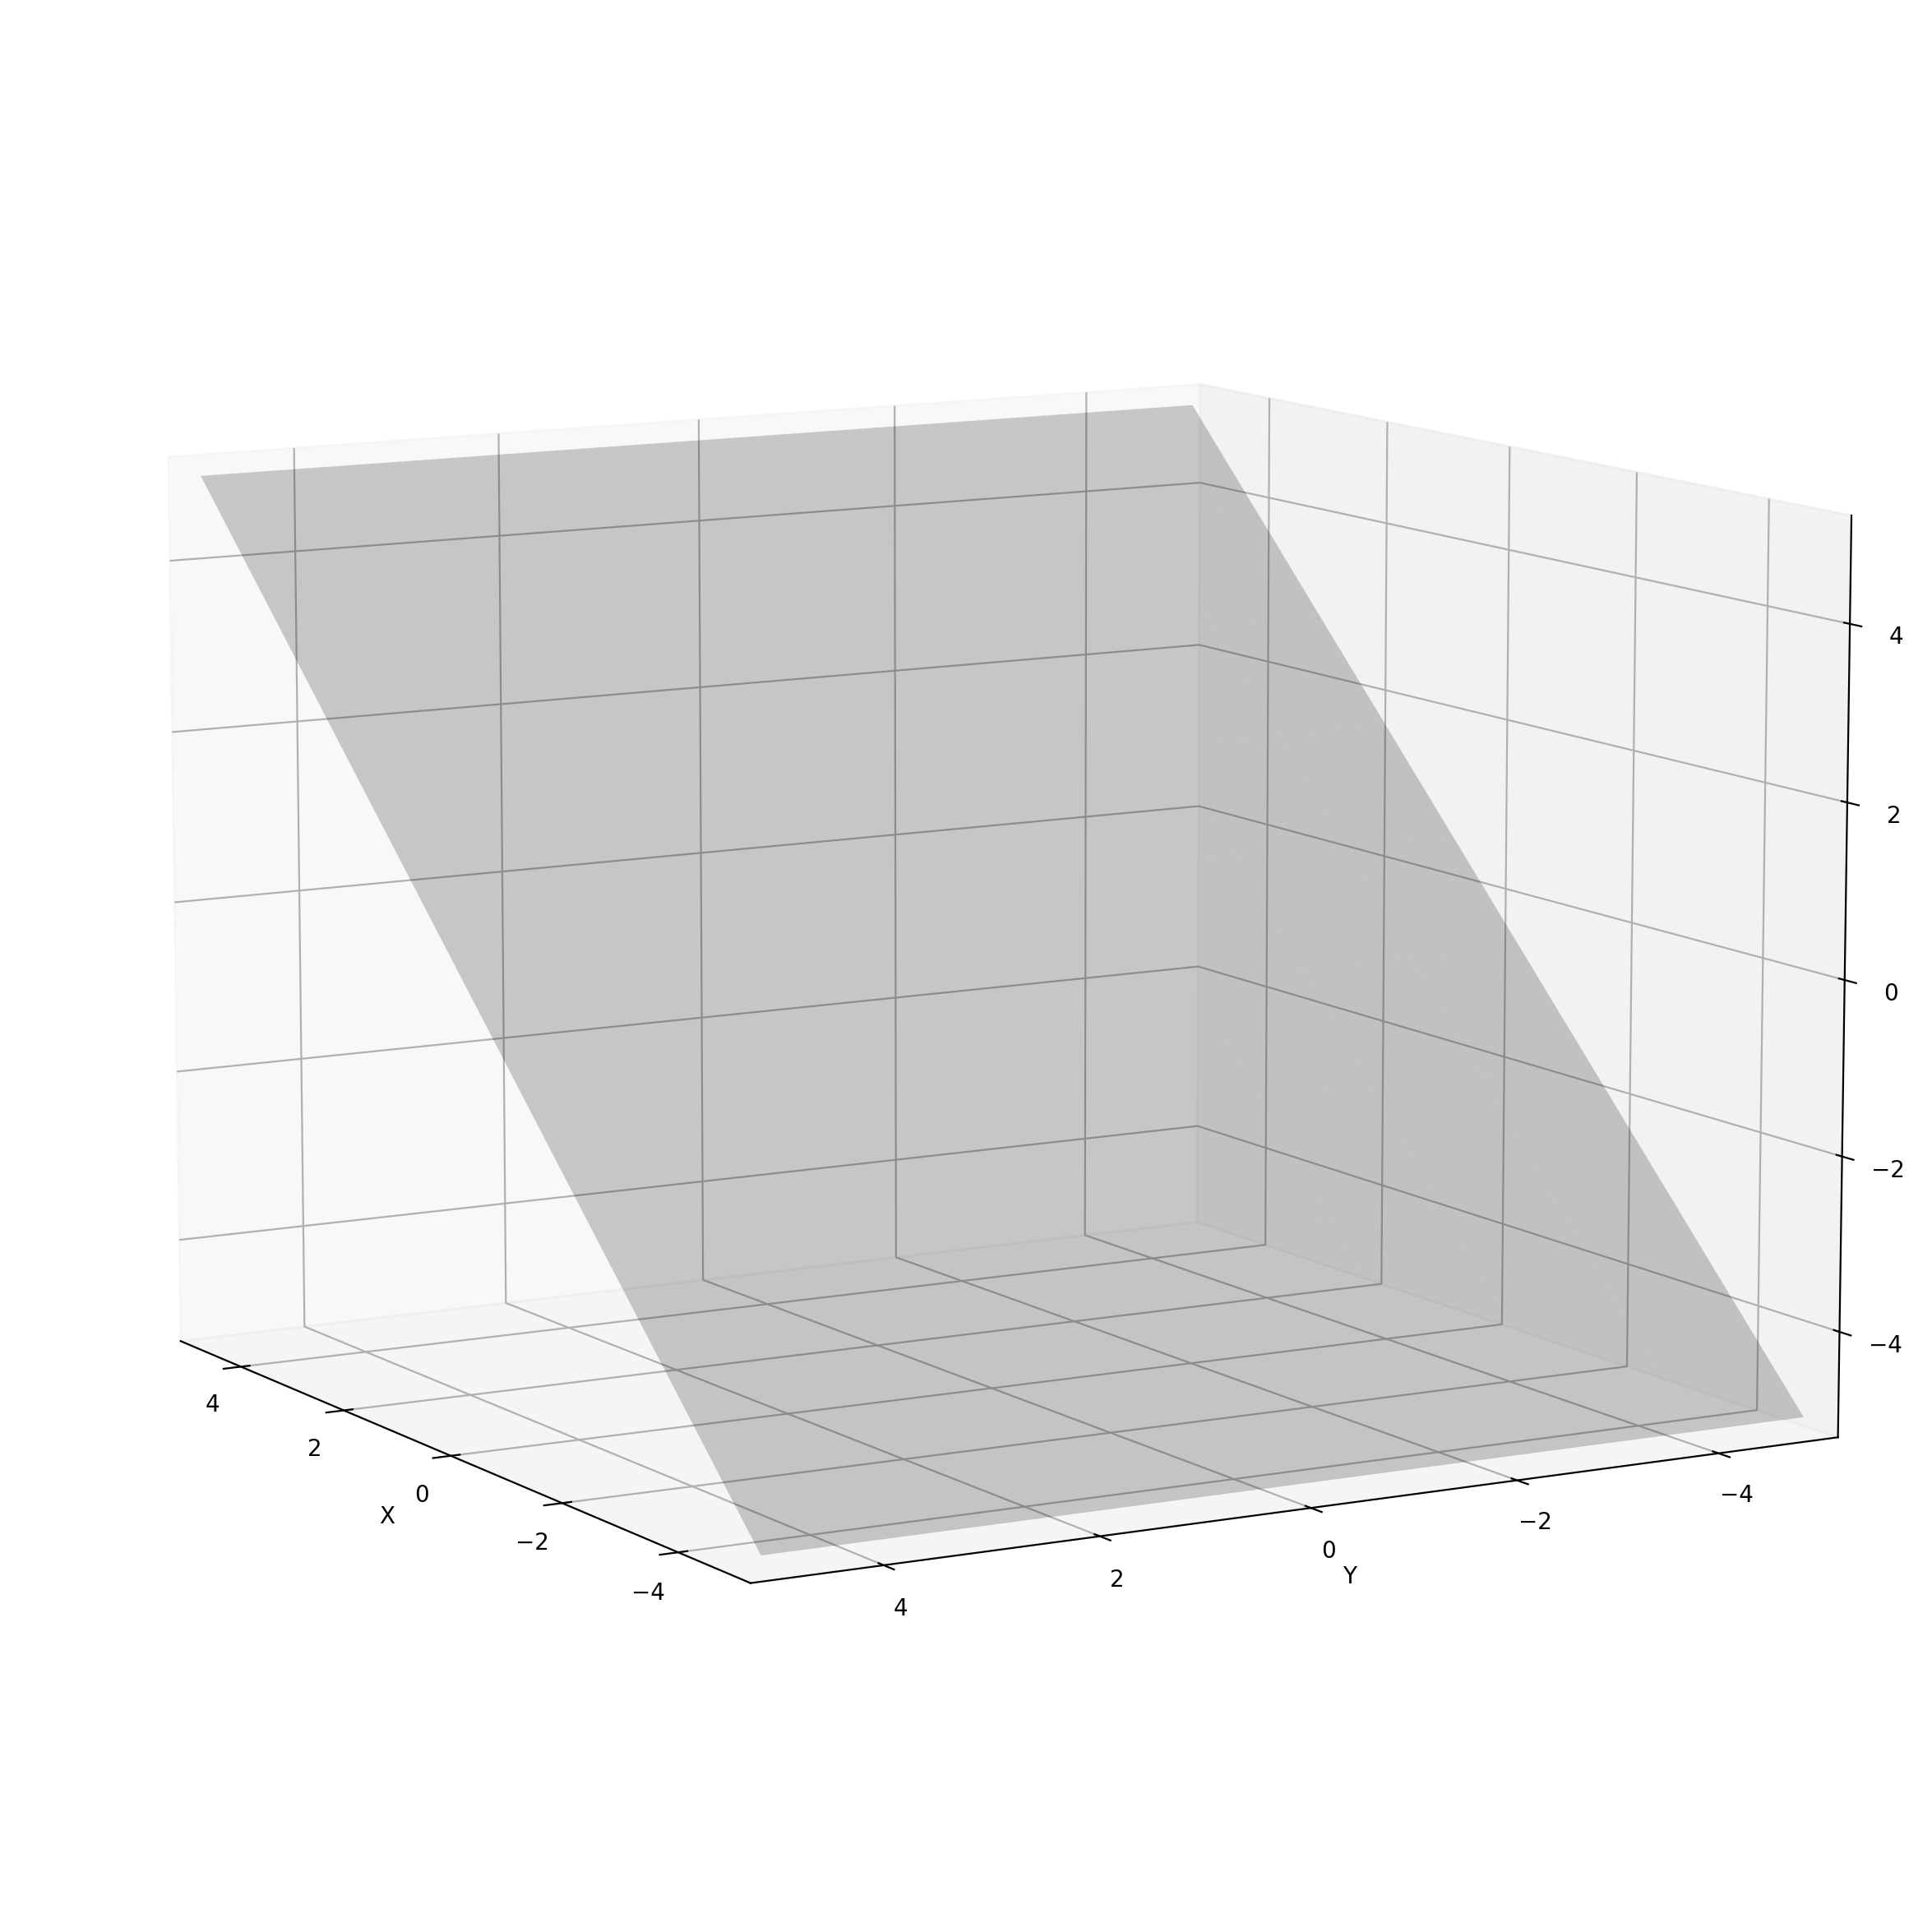
\includegraphics[scale=0.39]{Images/vector-space-ex.png}
    \caption{Graphical representation of $V$ vector space.}
    \label{fig:vector-space-ex}
\end{figure}
%%%%%%%%%%%%%%%%%%%%%%%%%%%%%%%%%%%%%%%%%%VECTOR-SUBSPACE%%%%%%%%%%%%%%%%%%%%%%%%%%%%%%%%%%%%%%%%%%%%%%%%%
\subsection{Vector Subspaces}

Let $V$ be a vector space over a field $\mathbb{F}$, and let $W$ be a non-empty subset of $V$. $W$ is called a \emph{vector subspace} of $V$ if it satisfies the following properties:

\begin{enumerate}
    \item \textbf{Closure under Vector Addition:} For any $\vec{u}, \vec{v} \in W$, their sum $\vec{u} + \vec{v}$ is also in $W$.
    
    \item \textbf{Closure under Scalar Multiplication:} For any $\vec{v} \in W$ and any scalar $c \in \mathbb{F}$, the scalar product $c\vec{v}$ is in $W$.
    
    \item \textbf{Contains the Zero Vector:} The zero vector $\vec{0}$ of $V$ is in $W$.
\end{enumerate}

If these conditions are met, $W$ is a vector subspace of $V$ and is denoted as $W \subseteq V$.
\\

\textbf{Example of Vector Subspace}

Consider \(W\) as a vector subspace of previously defined space \(V\):

$$
\scalebox{1.1}{$W \subseteq V = \{\vec v \in \mathbb{R}^3 \ | \ v_3 = v_1\}$}
$$$$
\scalebox{1.1}{$W = \{ \vec{w} \in \mathbb{R}^3 \mid w_3 = w_1 \land w_1 + w_2 = 0\}$}
$$

In other words, \(W\) consists of all vectors in \(\mathbb{R}^3\) whose component $w_3$ is equal to $w_1$ and $w_1$ and $w_2$ components sum to zero.
\\

Let's check the three conditions for \(W\) to be a vector subspace:

\begin{enumerate}
    \item \textbf{Closure under Addition:}
     \begin{itemize}
            \item Take \(\vec{v} =\begin{bmatrix} v_1 \\ -v_1 \\ v_1 \end{bmatrix}\) and \(\vec{w} =\begin{bmatrix} w_1 \\ -w_1 \\ w_1 \end{bmatrix}\) where \(\vec v, \vec w \in W \).
            \item Their sum \(\vec{v} + \vec{w} =\begin{bmatrix} v_1 + w_1 \\ -(v_1 + w_1) \\ v_1 + w_1 \end{bmatrix} = \vec z\) is also in \(W\) because \(z_2 = -z_1 \land z_3 = z_1\).
        \end{itemize}
        
    \item \textbf{Closure under Scalar Multiplication:}
     \begin{itemize}
            \item Take \(\vec{w} =\begin{bmatrix} w_1 \\ -w_1 \\ w_1 \end{bmatrix} \in W\) and \(k \in \mathbb{R}\).
            \item The scalar multiple \(k \cdot \vec{w} =\begin{bmatrix} kw_1 \\ -(kw_1) \\ kw_1 \end{bmatrix} = \vec z\) is also in \(W\) since \(z_1 = -z_2 \land z_3 = z_1\).
        \end{itemize}
    
    \item \textbf{Contains the Zero Vector:}
     \begin{itemize}
            \item The zero vector \(\vec{0} =\begin{bmatrix} 0 \\ 0 \end{bmatrix}\) is in \(W\) because \(z_1 = -z_2 \land z_3 = z_1\).
        \end{itemize}
\end{enumerate}
Therefore, \(W\) satisfies all conditions and is indeed a vector subspace of \(V\).
\\

The graphical representation of the vector subspace $W$ is a one-dimensional line as shown in Figure \ref{fig:vector-subspace-ex}.
\begin{figure}[h]
    \centering
    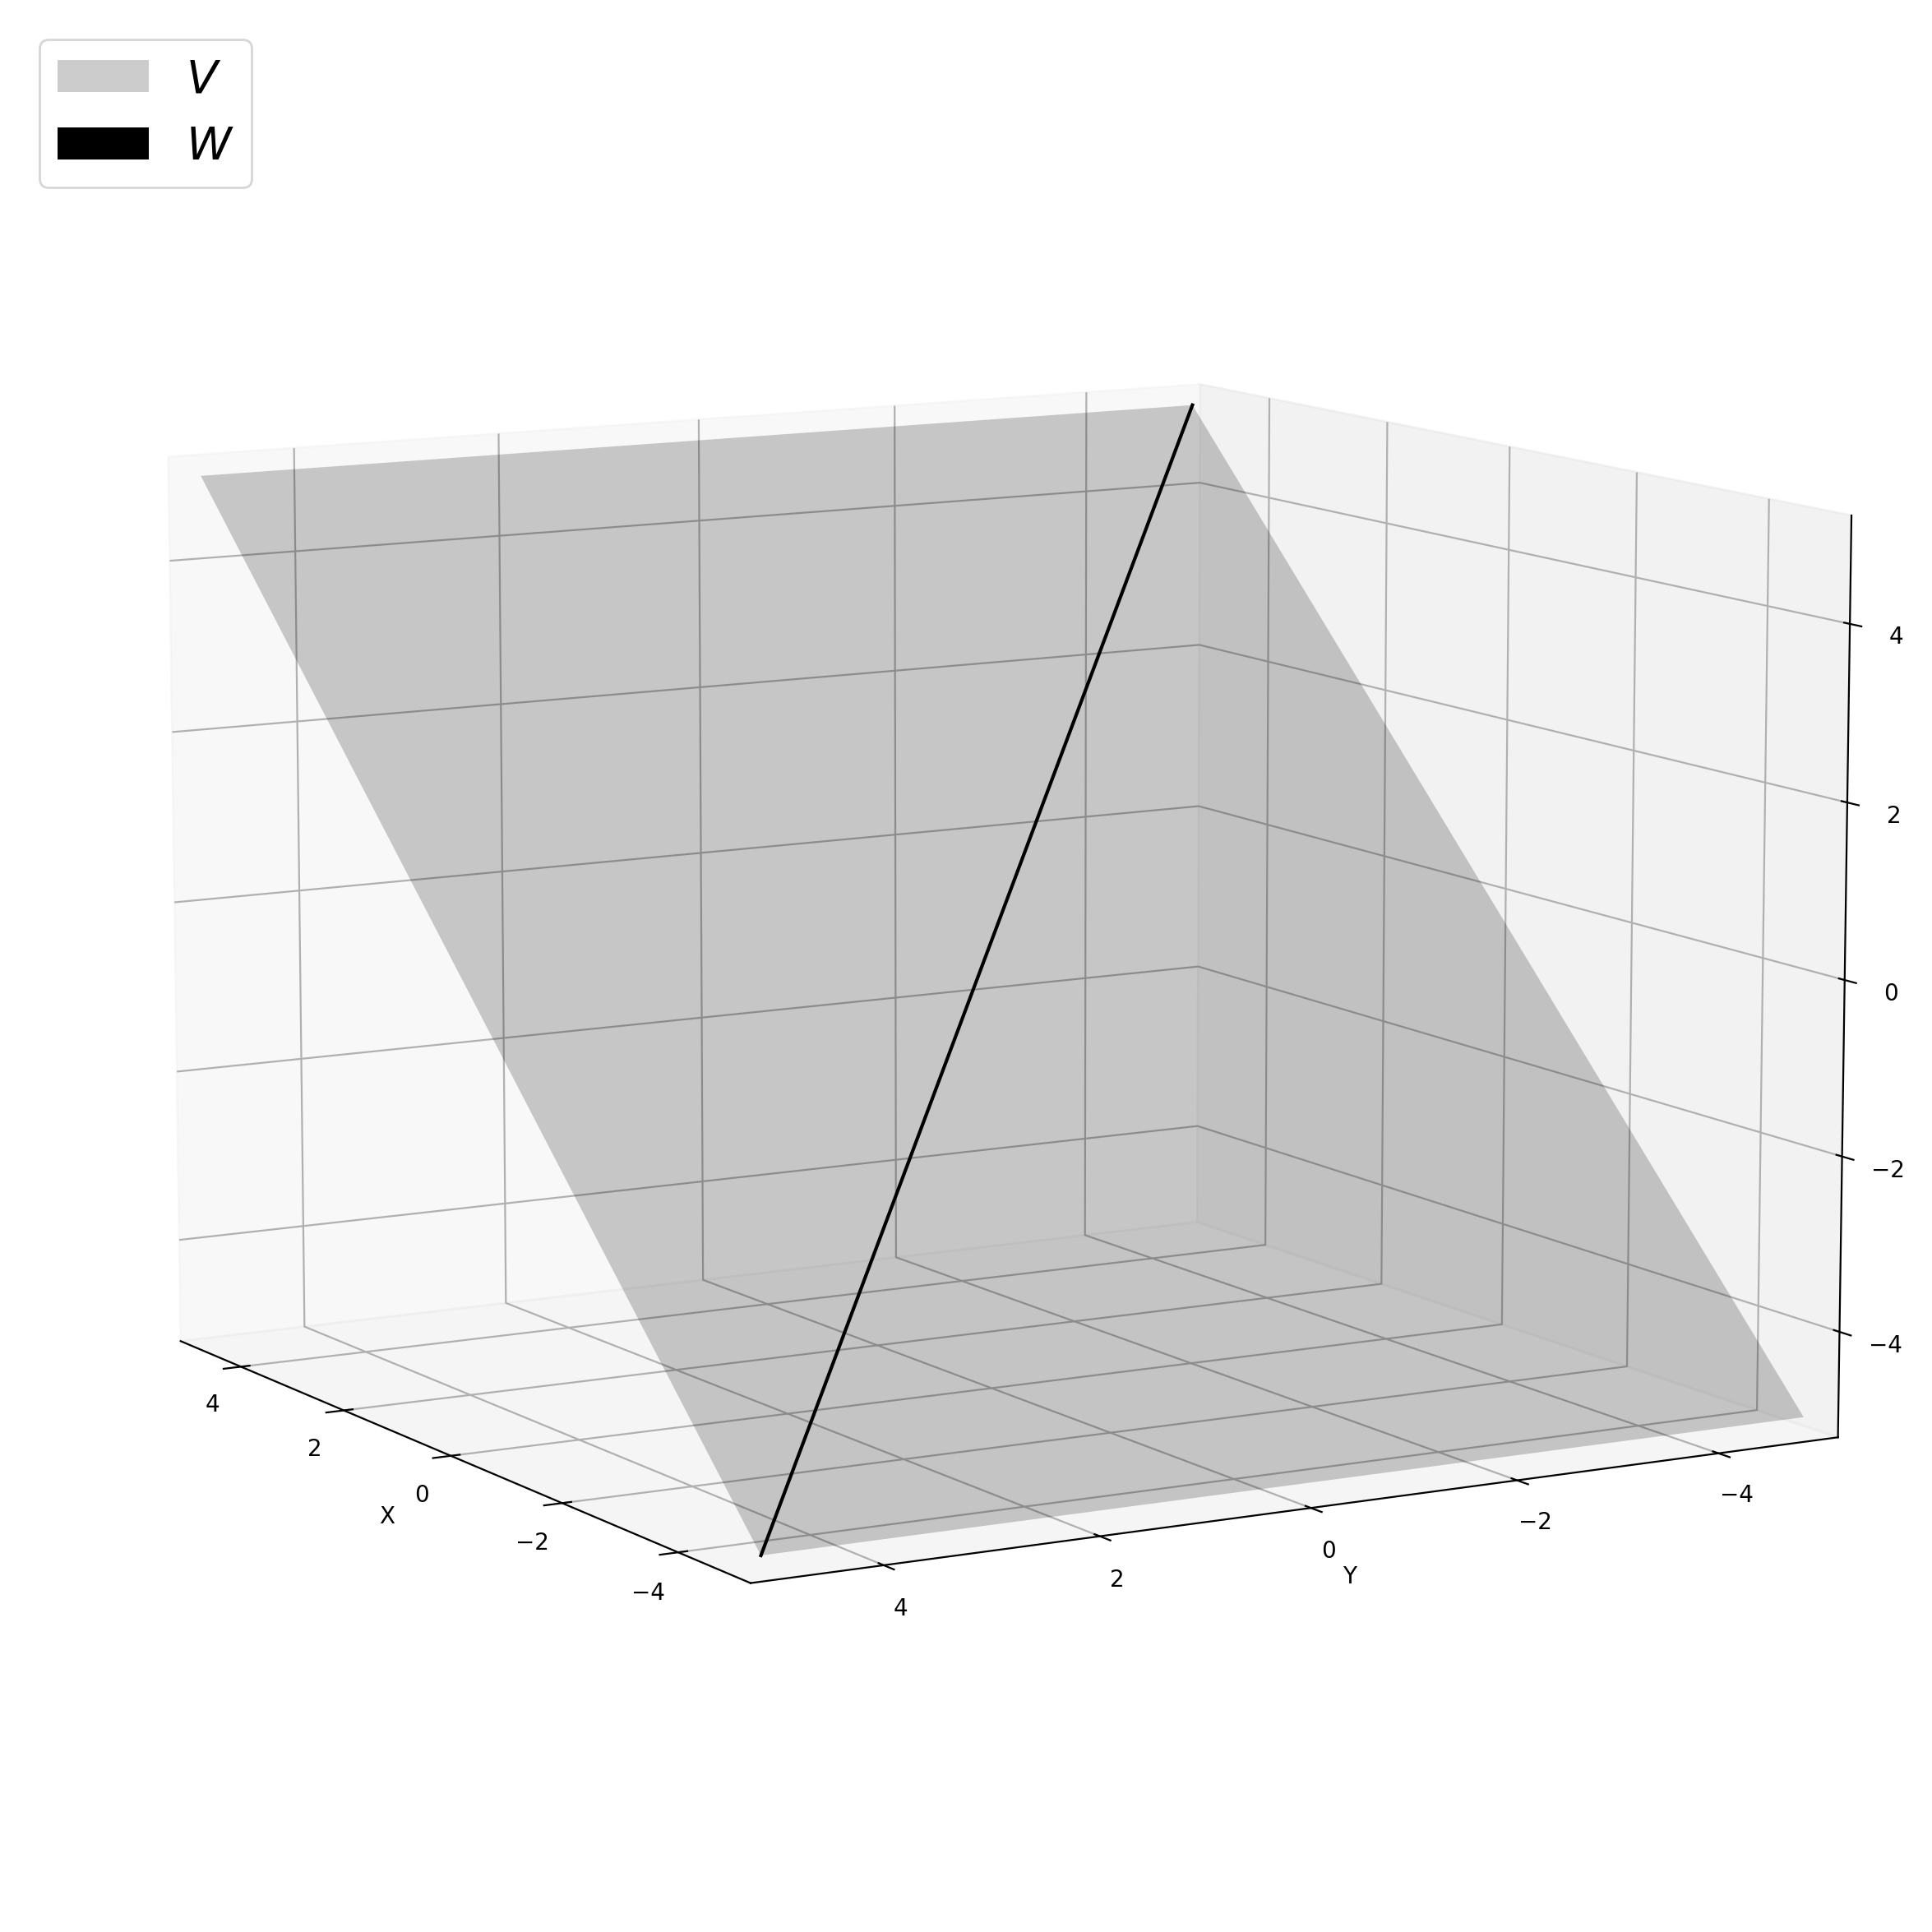
\includegraphics[scale=0.36]{Images/vector-subspace-ex.png}
    \caption{Graphical representation of $V$ vector space (gray) and $W$ vector subspace (black).}
    \label{fig:vector-subspace-ex}
\end{figure}
\newpage
\section{Linear Combinations}

In the realm of vector spaces, the concept of a \emph{linear combination} holds significant importance. A \emph{linear combination} involves combining vectors in a space by scaling each vector by a scalar and then summing them up. 


    Let $V$ be a vector space over the field $\mathbb F$. If $\vec{v}_1, . \ . \ ., \vec v_s \in V$ are vectors and $a_1, . \ . \ ., a_s \in \mathbb F$ are scalars, then the \textbf{linear combination} of those vectors with those scalars as coefficients is 

$$
a_1 \vec v_1 + \dots + a_s \vec v_s \ \in V, \quad a_1, . \ . \ ., a_s \in \mathbb F.
$$

\label{def:linear-combination}



Understanding linear combinations is foundational in linear algebra, providing insights into the structure and properties of vector spaces. Linear combinations play a crucial role in defining concepts such as span, linear independence, and solutions to systems of linear equations.
%%%%%%%%%%%%%%%%%%%%%%%%%%%%%%%%%%%%%%%%%%SPAN%%%%%%%%%%%%%%%%%%%%%%%%%%%%%%%%%%%%%%%%%%%%%%%%%
\subsection{Span}

The \textbf{span} of a nonempty subset $S$ of a vector space $V$ over a field $\mathbb F$, is the set of all possible linear combinations of those vectors.

$$
\textit{span}(\vec{v}_1, \vec{v}_2, \ldots, \vec{v}_k) = \left\{ \sum_{i=1}^k \lambda_i \vec{v}_i \ \middle| \ k \in \mathbb{N}, \vec{v}_i \in V, \lambda_i \in \mathbb F \right\}
$$

The span of the empty subset of a vector space is its trivial subspace.
\\

In simpler terms, the span is the set of all possible vectors that can be formed by linear combinations of the given vectors.
\\

Let $S \subseteq V$. The set $S$ is a \textbf{spanning set} of $V$ if \textit{every} $\vec v \in V$ can be written as linear combination of vectors in $S$.


\subsubsection{The Span of a Subset of a Vector Space is a Vector Subspace}

Let $S$ be a set of vectors of vector space $V$. The {\textit{span($S$)}} is a vector subspace.
\\

\textbf{\textit{Proof}}
\\

Let's show that \textit{span}($S$) is a vector space. 

Let $S$ be a subset of $V$, if $S$ = $\emptyset$ it is the trivial vector space. If $S \neq \emptyset$ then $S = \{\vec s_1, \dots , \vec s_n\}$ and two generic vector of \textit{span}($S$) are written as 

\begin{align*}
\vec w &= \lambda_1 \vec s_1 + \dots + \lambda_n \vec s_n\\
\vec v &= \gamma_{1} \vec s_1 + \dots + \gamma_{n} \vec s_n
\end{align*}

So the sum $\vec v + \vec w = (\lambda_1 + \gamma_1) \vec s_1 + \dots + (\lambda_n + \gamma_n) \vec s_n$ is an element of \textit{span}($S$).
\\

Now we have to prove that \textit{span}($S$) is close under multiplication by a scalar.
\\

Consider again the vector $\vec w = \lambda_1 \vec s_1 + \dots + \lambda_n \vec s_n$ and a generic scalar $r$.

$$
r \cdot \vec w = r \cdot (\lambda_1 \vec s_1 + \dots + \lambda_n \vec s_n) = r\lambda_1 \vec s_1 + \dots + r\lambda_n \vec s_n
$$

That is a linear combination of vectors in $S$, so $r \cdot \vec w \in \textit{span}(S)$.

All the other axioms are inherited from $V$. $\blacksquare$
\\

The span plays a crucial role in determining the extent or reach of a set of vectors. If the span of a set of vectors is the entire vector space $V$, then the vectors are said to \emph{span} the space.
%%%%%%%%%%%%%%%%%%%%%%%%%%%%%%%%%%%%%%%%%%LINEAR-INDEPENDENCE%%%%%%%%%%%%%%%%%%%%%%%%%%%%%%%%%%%%%%%%%%%%%%%%%
\section{Linear (in)dependence}

    In a vector space $V$, a subset of vectors is deemed \emph{linearly independent} if no vector within the subset can be expressed as a linear combination of others in the same subset. Conversely, if such a linear combination exists, the subset is \emph{linearly dependent}.

\begin{lemma}
   A subset $S$ of a vector space $V$ is linearly independent if, and only if, the only linear combination among its elements that results in the zero vector is the trivial one:

   $$
   c_1 \vec s_1 + \dots +, c_n \vec s_n = \vec 0, \quad \text{with} \ c_1 = \dots = c_n = 0 
   $$

where $s_i \neq s_j$ when $i \neq j$.
\end{lemma}


\textbf{\textit{Proof}}\\
$\implies$
\\
$S$ is a \textit{linearly independent} set. Suppose, for the sake of contradiction, that there exists a nontrivial linear combination of the elements of $S$ that results in the zero vector. Then, there exists a finite subset ${\vec s_1, \vec s_2,..., \vec s_n}$ of $S$ and scalars $c_1,c_2,...,c_n$, not all zero, such that

$$
c_1 \cdot \vec s_1 + c_2 \cdot \vec s_2 + \cdots + c_n \cdot \vec s_n = 0
$$

This implies that at least one of the scalars is nonzero, say $c_1 \neq 0$, and the above equation is able to be written as

$$\vec{s}_1 = -\frac{c_2}{c_1} \vec{s}_2 + \cdots + -\frac{c_k}{c_1} \vec{s}_k,$$

if $k > 1$, and $\vec{s}_1 = \vec{0}$ if $k = 1$.
\\

We have just written a vector in $S$ as a linear combination of other vectors in $S$. But $S$ is a \textit{linearly dependent} set. $\bot$\\

$\notimplies$

If $S$ is not \textit{linearly independent} then some $\vec s_i$ is a linear combination of other vectors in $S$, so 

$$
\vec s_i = c_1 \vec s_1 + \dots + c_{i-1} \vec s_{i-1} + c_{i+1} \vec s_{i+1} + \dots + c_{n} \vec s_n
$$

Subtracting $\vec s_i$ from both sides, gives a relationship involving a nonzero coefficient (-1 in front of $\vec s_i$).

$$
\vec 0 = c_1 \vec s_1 + \dots + -1 \cdot \vec s_i + \dots + c_{n} \vec s_n.
$$

So the linear combination is not the trivial one. $\blacksquare$
\\

Thus, a set of vectors is \emph{linearly dependent} if and only if one of them is zero or a linear combination of the others.

\begin{lemma}
    Let $V$ be a vector space, $S \subseteq V$ and $\vec v \in V$. 
    
    $$\textit{span}{\normalfont (S \cup \{\vec v\}) = \textit{span}(S)} \iff \vec v \in \textit{span}{\normalfont (S)}
    $$
\end{lemma}


\textbf{\textit{Proof}} 

$\implies$

If $\vec v \notin \textit{span}(S) \iff \textit{span}{\normalfont (S \cup \{\vec v\}) \neq \textit{span}(S)}$, so $\textit{span}{\normalfont (S \cup \{\vec v\}) = \textit{span}(S)} \implies \vec v \in \textit{span}{\normalfont (S)}$

$\!\impliedby$

It is clear that $\textit{span}(S) \subseteq \textit{span}{\normalfont (S \cup \{\vec v\})}$.
\\

Let be $S = \{s_1, \dots, s_n\}$.

If $\large \vec v \in \textit{span}(S) \implies \vec v = \sum_{i = 1}^{n} \lambda_{i+n} \vec s_i$, so 
we can express a generic vector $\vec w \in \textit{span}(S \cup \{\vec v\})$ as a linear combination of
vectors in $S$ in this form:

$$
\vec w = \lambda_1 \vec s_1 + \dots \lambda_n \vec s_n + k \vec v
$$
$$
\vec w = \lambda_1 \vec s_1 + \dots \lambda_n \vec s_n + k(\lambda_{n+1} \vec s_1 + \dots \lambda_n \vec s_{n+n})
$$
$$
\vec w = (\lambda_1 + k\lambda_{n+1}) \vec s_1 + \dots + (\lambda_n + k\lambda_{n+n}) \vec s_n
$$

Thus the generic vector $\vec w \in \textit{span}(S \cup \{\vec v\})$ is also in $\textit{span}(S)$ because it is a linear combination of vectors in $S$, so $\textit{span}{\normalfont (S \cup \{\vec v\})} \subseteq \textit{span}(S)$, so $\textit{span}{\normalfont (S \cup \{\vec v\})} = \textit{span}(S)$. $\blacksquare$

\begin{corollary}
    Let $V$ be a set of vectors and $\vec v \in V$, \textit{span}{\normalfont ($V$) = \textit{span}($V \setminus \{\vec v\}$)} if and only if $\vec v$ is dependent on other vectors in the set $V$.
    \label{cor:same-span}
\end{corollary}


\textbf{\textit{Proof}} 

$\implies$

If $\vec v \in V$ then $\vec v \in \textit{span}(V)$. Since $\textit{span}(V) = \textit{span}(V \setminus \{\vec v\})$ so $\vec v \in \textit{span}(V \setminus \{\vec v\})$, and so $\vec v = \lambda_1 \vec v_1 + \dots + \lambda_n \vec v_n$. That implies that $\vec v$ is dependent on vectors in $V \setminus \{\vec v\}$.

$\!\impliedby$

If $\vec v \in \textit{span}(V \setminus \{\vec v\})$ then $\vec v = \lambda_1 \vec v_1 + \dots + \lambda_n \vec v_n$, so $\vec v$ is also in \textit{span}$(V)$. $\blacksquare$
\\

The corollary asserts that if the removal of a vector from a set don't reduce the span, then that vector is a linear combination of some other vectors in that set.

\begin{corollary}
    A set $S$ is linearly independent if and only if, for any $\vec{v} \in S$, its removal shrink the span $\text{span}(S - \{\vec{v}\}) \subset \text{span}(S)$.
\end{corollary}


\textbf{\textit{Proof}} If $S$ is linearly independent then the removal of a vector will shrink the \textit{span}($S$) (for corollary \ref{cor:same-span}). If $S$ is not linearly independent then the removal of a vector will not shrink the \textit{span}($S$). $\blacksquare$
\\

\begin{lemma}
    Let $V$ be a linearly independent set of vectors, and let $\vec v \notin V$. Then 
    the set $V \cup \{\vec v\}$ is linearly independent if and only if $\vec v \notin \textit{span}(V)$.
\end{lemma}


\textbf{\textit{Proof}}

$\implies$

If $V \cup \{\vec v\}$ is a linear independent set, then $\vec v$ is not a linear combination of vectors in $V$. So  $\vec v \notin \textit{span}(V)$.

$\!\impliedby$

If $\vec v \notin \textit{span}(V)$ then $\vec v$ is not a linear combination of vectors in $V$, so if $V$ is all linear independent set, then also $V \cup \{\vec v\}$ is.
$\blacksquare$


\begin{corollary}
    In a vector space, every finite set of vectors possesses a linearly independent subset with the same span.
\end{corollary}


\textbf{\textit{Proof}} Let $V$ be a vector space, and $S = \{\vec s_1, \dots, \vec s_n\}$ be a subset of it. If the set $S = \{\vec s_1, \dots, \vec s_n\}$ is linear independent then $S$ itself satisfies the statement. Else, let's remove iteratively from $S$ each vector that is a linear combination of other, until we obtain a subset $K \subset S$ that is linearly independent. $K$ is a linearly independent subset
with the same span of $S$.
$\blacksquare$


\begin{corollary}
    A subset $S = \{\vec s_1, \dots, \vec s_n\}$ of a vector space $V$ is linearly dependent if and only if some $\vec s_i \in S$ is a linear combination of other vectors in $\{\vec s_1, \dots, \vec s_{i-1}\}$ listed before it.
\end{corollary}


\textbf{\textit{Proof}} 

Consider $S_0 = \{ \}, \ S_1 = \{\vec s_1 \}, \ S_2 = \{\vec s_1 , \vec s_2 \}$, etc. Some index $i \geq 1$ is the
first one with $S_{i−1} \cup \{\vec s_i \}$ linearly dependent, and there $\vec s_i \in \textit{span}(S_{i−1})$.
$\blacksquare$

\begin{lemma}
    Any subset of a linearly independent set is also linearly independent.
Any superset of a linearly dependent set is also linearly dependent.
\end{lemma}


\textbf{\textit{Proof}} Both are clear.

%%%%%%%%%%%%%%%%%%%%%%%%%%%%%%%%%%%%%%%%%%BASIS%%%%%%%%%%%%%%%%%%%%%%%%%%%%%%%%%%%%%%%%%%%%%%%%%
\section{Basis and Dimension}

\subsection{Basis}

A maximal linearly independent subset of vectors of $V$ that spans $V$ is called a \textbf{basis} of the vector space $V$.
\\

This means that a subset $B$ of $V$ is a \textbf{basis} if it satisfies the two following conditions:

\begin{itemize}
\item \textbf{Linear independence:}
    For every finite subset $\{ \vec{\beta} _{1},\dotsc ,\vec {\beta}_{n}\}$ of $B$, if ${\displaystyle c_{1}\vec {\beta}_{1} + \cdots + c_{n}\vec {\beta}_{n}=\vec {0} }$ for some ${\displaystyle c_{1},\dotsc ,c_{m}}$ in $\mathbb F$, then ${\displaystyle c_{1}=\cdots =c_{m}=0}$.
\item \textbf{Spanning property:}
    For every vector $\vec{v}$ in $V$, one can choose ${\displaystyle a_{1},\dots, a_{n}}$ in $\mathbb F$ and ${\displaystyle \vec {\beta}_{1},\dots  ,\vec {\beta}_{n}}$ in $B$ such that ${\displaystyle \vec {v} = a_{1}\vec {\beta}_{1} + \cdots + a_{n}\vec {\beta}_{n}}$.
\end{itemize}

The scalars $a_{i}$ are called the coordinates of the vector $\vec{v}$ with respect to the \textbf{basis} $B$, and by the first property they are uniquely determined.
\\

Note that is more useful to consider a basis as a sequence of vectors instead of a set. This because when considering the coordinates of a vector, we have an implicit need to know the order of the basis vectors for applying coordinates to the right basis vectors. For this reason, we will denote a basis with angle brackets $\langle \beta_1, \beta_2, \dots, \beta_n \rangle$.
\\

We can view a basis of a vector space as a minimal subset of vectors with which we can control all the dimensions of a vector space. In particular, each vector in the basis is responsible for "controlling" one dimension of the vector space. This way, through coefficients, we can express each dimension of the vector space. From the perspective of an individual component of a vector: the basis vector responsible for the $i$-th component of vector $\vec{v}$ will be a vector from the basis (let's denote it for simplicity as $\vec{\beta}_x \in B$). In this case, the $i$-th component of the basis vector $\vec{\beta}_x$ and the coefficient $\alpha_x$ will be responsible for generating the $i$-th component of vector $\vec{v}$ in a similar way to this: $v_i = \alpha_x b_{x_i}$.
\\

However, since there are other combinations that indirectly affect the same dimension managed by the basis vector $\vec{\beta}_x$, we also need to include these coefficients in the equation. Thus, we obtain $v_i = \alpha_1 \vec\beta^i_{1} + \ldots + \alpha_x \vec{\beta}^i_{x} + \ldots + \alpha_n \vec{\beta}^i_{n}$. Therefore, to find all the coefficients of the basis for vector $\vec{v}$ (across all components), one needs to solve the linear system $v_i = \alpha_1 \vec{\beta}^i_{1} + \ldots + \alpha_x \vec{\beta}^i_{x} + \ldots + \alpha_n \vec{\beta}^i_{n}$ for each $i$ from $1$ to $n$.

$$
\begin{cases}
\alpha_1 \vec{\beta}^1_{1} + \ldots + \alpha_x \vec{\beta}^1_{x} + \ldots + \alpha_n \vec{\beta}^1_{n} = v_1 \\
\ \ \vdots\\
\alpha_1 \vec{\beta}^n_{1} + \ldots + \alpha_x \vec{\beta}^n_{x} + \ldots + \alpha_n \vec{\beta}^n_{n} = v_n
\end{cases}
$$

And since it is a linear system of $n$ equations and $n$ variables (where all equations are linearly independent, as we mentioned that ${B}$ is a minimal set that can control all dimensions of $V$), we obtain a unique solution for each vector in $V$.


For each $\mathbb{R}^n$ vector space, the vectors 

$$\xi_n = \langle \begin{bmatrix} 1 \\ 0 \\ 0 \\ \vdots \\ 0\end{bmatrix}, \\ \begin{bmatrix} 0 \\ 1 \\ 0 \\ \vdots \\ 0\end{bmatrix}, \ \dots, \\\begin{bmatrix} 0 \\ 0 \\ 0 \\ \vdots \\ 1\end{bmatrix}\rangle$$ 

are a \textbf{basis} (known as \emph{canonical} \textbf{basis}) also known as $\xi_n$. We denote these vectors $\vec{e}_1, \dots, \vec{e}_n$.



\begin{theorem}
In a vector space $V$, a subset is a basis if and only if each vector
in the space can be expressed as a linear combination of elements of the subset
in one and only one way.

\label{the:unique-lc-basis}
\end{theorem}

\textbf{\textit{Proof}}

$\implies$

$B$ is a basis of $V$ space, so each vector $\vec v \in V$ is a linear combination of vectors in $B$. We now prove that the coordinates of the combination are unique for each vector in $V$.

If for absurdity there exist two linear combinations such that

$$
\vec v = a_1 \vec \beta_1 + \dots + a_n \vec \beta_n = c_1 \vec \beta_1 + \dots + c_n \vec \beta_n
$$
then

$$
(a_1 - c_1) \vec \beta_i + \dots + (a_n - c_n) \vec \beta_n = \vec 0
$$

Since the vectors in $B$ are a basis (a linear independent set), the only way to get vector $\vec 0$ is the trivial one, so all the coefficients $a_i$ must be equal to $c_i$, so there exists only one linear combination for each vector in $V$.

$\!\impliedby$

Since each vectors in $V$ can be expressed as a linear combination of vectors in $B$ in one and only one way, then we have to prove that all vectors $\vec \beta_i \in B$ are linearly independent.

If there exists a vector $\vec \beta_i \in B$ that is a linear combination of other vectors in $B$, then

$$
\vec \beta_i = \lambda_1 \vec \beta_i + \dots + \lambda_{i-1} \vec \beta_{i-1} + \lambda_{i+1} \vec \beta_{i+1} + \dots + \lambda_n \vec \beta_n
$$

But we also know that there exists an other linear combination of vectors in $B$ that generate $\vec \beta_i$, that is different from the previous one:

$$
\vec \beta_i = 0 \cdot \beta_1 + \dots + 1 \cdot \beta_i + \dots + 0 \cdot \beta_n
$$

However we can have just one linear combination for each vector in $V$. $\bot$
\\

In this way we have proved that $B$ is an independent set and, consequently, that the theorem \ref{the:unique-lc-basis} is valid. $\blacksquare$
\\

In a vector space $V$ with a basis $B = \langle\vec \beta_1, \dots, \vec \beta_n \rangle$, the coordinates of a generic vector $\vec v \in V$ are the coefficients used to express $\vec v$ as a linear combinations of the basis vectors. So the coordinates of the vector $\vec v \in V$ with respect to basis $B$ are represented by the column vector 

$$
[\vec v]_B =\begin{bmatrix}
    c_1 \\
    \vdots\\
    c_n
\end{bmatrix}
$$



In a vector space, the coordinates of a vector with respect to a given \emph{basis} are unique. Specifically, let $V$ be a vector space and $B = \langle \vec{\beta}_1, \vec{\beta}_2, \ldots, \vec{\beta}_n\rangle$ be a \emph{basis} for $V$. For any vector $\vec{v} \in V$, there exists a unique set of scalars $c_1, c_2, \ldots, c_n$ such that:

$$
\vec{v} = c_1 \vec{\beta}_1 + c_2 \vec{\beta}_2 + \ldots + c_n \vec{\beta}_n
$$

This uniqueness property ensures that the coordinates of $\vec{v}$ in terms of the \emph{basis} $B$ are well-defined and distinct.
\\

For a given basis $B$ of $V$ with $n$ elements, a linear combination of vectors $a_1 \vec v_1 + \cdots + a_k \vec v_k= \vec 0$ if and only if $a_1 [\vec v_1]_B + \cdots + a_k [\vec v_k]_B = \vec 0$.

\begin{lemma}
    For a given basis $B$ of $V$ with $n$ elements, a linear combination of vectors $a_1 \vec v_1 + \cdots + a_k \vec v_k= \vec 0$ if and only if $a_1 [\vec v_1]_B + \cdots + a_k [\vec v_k]_B = \vec 0$.
\end{lemma}

\textbf{\textit{Proof}}

Let $\langle \vec \beta_1, \cdots, \vec \beta_n \rangle$ be a basis of $V$ vector space. Each vector $\vec v_i \in V$ can be expressed as a linear combination of basis vector, so:

\begin{align*}
a_1 \vec v_1 + \cdots + a_k \vec v_k &= a_1 (\alpha_{1,1} \vec \beta_1 + \cdots + \alpha_{1,n} \vec \beta_n) + \cdots + a_k (\alpha_{k,1} \vec \beta_1 + \cdots + \alpha_{k,n} \vec \beta_n) = \\
&=(a_1 \alpha_{1,1} + \cdots + a_k \alpha_{k,1}) \vec \beta_1 + \cdots + (a_1 \alpha_{1,n} + \cdots + a_k \alpha_{k,n}) \vec \beta_n = \vec 0.
\end{align*}

This implies that

$$
\begin{cases}
a_1 \alpha_{1,1} + \cdots + a_k \alpha_{k,1} = 0 \\
\ \ \vdots\\
a_1 \alpha_{1,n} + \cdots + a_k \alpha_{k,n} = 0
\end{cases}
$$

that can be easily written as follow:

$$
a_1 \begin{bmatrix}
\alpha_{1,1}\\
\vdots\\
\alpha_{1,n}
\end{bmatrix} + \cdots + a_{k} \begin{bmatrix}
\alpha_{k,1}\\
\vdots\\
\alpha_{k,n}
\end{bmatrix}
= a_1 [\vec v_1]_B + \cdots + a_k [\vec v_k]_B = \vec 0.
$$
$\blacksquare$

Geometrically, the whole matter can be interpreted in this way: each coordinate vector of every vector in the initial linear combination is "telling" how much "force" to apply to each base vector that "controls" a certain coordinate. Let's take an example: consider a generic component of every vector in the initial combination. We know that the combination $a_1 v_i + \cdots + a_k \cdot v_i$ equals zero, which tells us that the forces acting on the $i$-th component of the combination cancel out. However, this component (and all other components) stem from a sum of a linear combination of the $i$-th components of the base vectors. This implies that the force applied to any generic component is equally expressed by the same base vectors. So, for example $6=3\cdot2$ and $3=3\cdot1$, the combination $2 \cdot 6 + (-4) \cdot 3 = 0$, so also $2 \cdot (3\cdot2) + (-4) \cdot (3\cdot1) = 0$; now you can note that the number $3$ is our basis number, it can express $3$ and $6$.
The coordinate of $6$ is $2$ and the coordinate of $3$ is $1$. Substitute now $6$ with $3$ and $3$ with $1$ in the first combination and tah dah: $2 \cdot 2 + (-4) \cdot 1 = 0$. That is obvious because we have scaled the \textbf{same} basis number by two factors that cancel each other out.

\begin{lemma}
    {\normalfont \textbf{(Steinitz Lemma)}}
    Let U and W be finite subsets of a vector space V. If U is a set of linearly independent vectors, and W spans V , then: 
    \begin{enumerate}
        \item $|U| \leq |W|$.
        \item There is a set $W' \subseteq W$ with $|W'| = |W| - |U|$ such that $U \cup W'$ spans $V$.
    \end{enumerate}
    \label{lemma:steinitz}
\end{lemma}

\textbf{\textit{Proof}}

Suppose $U = \{ u_1, \ldots, u_m \}$ and $W = \{ w_1, \ldots, w_n \}$. We wish to show that $m \leq n$, and that after rearranging the $w_j$ if necessary, the set $\{ u_1, \ldots, u_m, w_{m+1}, \ldots, w_n \}$ spans $V$. We proceed by induction on $m$.
\\

For the base case, suppose $m$ is zero. In this case, the claim holds because there are no vectors $u_i$, and the set $\{ w_1, \ldots, w_n \}$ spans $V$ by hypothesis.

For the inductive step, assume the proposition is true for $m - 1$. By the inductive hypothesis, we may reorder the $w_i$ so that $\{ u_1, \ldots, u_{m-1}, w_m, \ldots, w_n \}$ spans $V$. Since $u_m \in V$, there exist coefficients $\mu_1, \ldots, \mu_n$ such that

\[
u_m = \sum_{i=1}^{m-1} \mu_i u_i + \sum_{j=m}^{n} \mu_j w_j.
\]
At least one of the $\mu_j$ must be non-zero, since otherwise this equality would contradict the linear independence of $\{ u_1, \ldots, u_m \}$; it follows that $m \leq n$. By reordering $\mu_m w_m, \ldots, \mu_n w_n$ if necessary, we may assume that $\mu_m$ is nonzero. Therefore, we have

\[
w_m = \frac{1}{\mu_m} \left( u_m - \sum_{j=1}^{m-1} \mu_j u_j - \sum_{j=m+1}^{n} \mu_j w_j \right).
\]
In other words, $w_m$ is in the span of $\{ u_1, \ldots, u_m, w_{m+1}, \ldots, w_n \}$. Since this span contains each of the vectors $u_1, \ldots, u_{m-1}, w_m, w_{m+1}, \ldots, w_n$, by the inductive hypothesis it contains $V$.

\begin{lemma}
{\normalfont\textbf{(Exchange Lemma)}}

Consider a vector space $V$ and a basis $B$ of $V$, then $\forall \vec v \in V$ (with $\vec v \neq \vec 0$)
the linear combination 

$$
\vec v = c_1 \vec \beta_1 + \dots + c_n \vec \beta_n
$$

has at least one coefficient $c_i \neq 0$. Then we can exchange $\vec \beta_i$ with $\vec v$ obtaining a set $B' = \langle \vec \beta_1, \dots, \vec \beta_{i-1}, \vec v, \vec \beta_{i+1}, \dots , \vec \beta_n\rangle$ that is another basis for $V$.
\label{lemma:exchange}
\end{lemma}


\textbf{\textit{Proof}}

We have to show that $B'$ is a basis for the vector space $V$. So $B'$ must be:

\begin{enumerate}
    \item a spanning set for $V$.
    \item a linearly independent set.
\end{enumerate}

1. We have to show that with the linear combination 

$$
\alpha_1 \vec \beta_1 + \dots + \alpha_{i-1} \vec \beta_{i-1} + \alpha_i \vec v + \alpha_{i+1} \vec \beta_{i+1} + \dots + \alpha_n \vec \beta_n
$$

we can generate all vectors in $V$. Remember that the vectors in $B$ are a spanning set for $V$. Let's now consider the vector $\vec v = c_1 \vec \beta_1 + \dots + c_n \vec \beta_n$.

By exchanging $\vec v$ with his linear combination expressed by the basis $B$ we obtain

$$
\alpha_1 \vec \beta_1 + \dots + \alpha_{i-1} \vec \beta_{i-1} + \alpha_i (c_1 \vec \beta_1 + \dots + c_n \vec \beta_n) + \alpha_{i+1} \vec \beta_{i+1} + \dots + \alpha_n \vec \beta_n =
$$
$$
= (\alpha_1 + \alpha_i c_1) \vec \beta_1 + \dots + \alpha_i c_i \vec \beta_i + \dots + (\alpha_n + \alpha_i c_n) \vec \beta_n
$$
that is a linear combination of vectors in basis $B$, so $B'$ can span all vectors in $V$ as well as $B$.
\\

2. We have to show that the vectors in $B'$ are all linear independent.

We already know that all vectors in $B$ are linearly independent. So also vectors in $B' \setminus \langle\vec v\rangle$ are independent.

So we have to show only that $\vec v$ is independent from vectors in $B' \setminus \langle\vec v\rangle$.

If $\vec v$ were a dependent vector, then there exists a way to write

$$
\vec v = c_1 \vec \beta_1 + \dots + c_{i-1} \vec \beta_{i-1} + c_{i+1} \vec \beta_{i+1} + \dots + c_n \vec \beta_n
$$
that means
$$
\vec v = c_1 \vec \beta_1 + \dots + c_{i-1} \vec \beta_{i-1} + 0 \vec \beta_i + c_{i+1} \vec \beta_{i+1} + \dots + c_n \vec \beta_n
$$

($0 \vec \beta_i$ because we have exchange $\vec b_i$ for $\vec v$).

But this contradicts the assumption $c_i \neq 0$, and since there is one and only one linear combination to write the vector $\vec v$ respect to vectors in $B$ basis, the only valid linear combination of vectors in $B$ has the coefficient $c_i \neq 0$. So also vector $\vec v$ is linearly
independent from other vectors in $B' \setminus \langle\vec v\rangle$. Thus $B'$ is a linear independent set. $\blacksquare$

\begin{theorem}
    All basis of a finite-dimensional vector space has the same number of elements.
\end{theorem}

\textbf{\textit{Proof}}

Suppose that $B_1=\langle \alpha_1, \cdots, \alpha_n \rangle$ and $B_2 = \langle \beta_1, \cdots, \beta_m \rangle$ are two bases of a vector space $V$.
\\

By \ref{lemma:steinitz} \textbf{(Steinitz Lemma)}, we know that $|B_1| \leq |B_2| \land |B_2| \leq |B_1|$. This implies $|B_1| = |B_2|$.
$\blacksquare$

\begin{theorem}
    Every set with more than $n$ vectors in a vector space $V$ of dimension $n$ or less is linearly dependent.
    \label{theo:every-set-with-more-than-n-elements-is-ld}
\end{theorem}

\textbf{\textit{Proof}}

Let $S = \{\vec{v}_1, \vec{v}_2, ..., \vec{v}_m\}$ be a set of $m$ vectors in a vector space $V$ of dimension $n$, where $m > n$; and let $B=\langle \beta_1, \cdots, \beta_n\rangle$ be a basis of $V$.

Suppose that $S$ is a linearly independent set. By the \ref{lemma:exchange} \textbf{Exchange Lemma} we can exchange $n$ vector in $B$ with a vector in $S$. But if $m>n$ there exists at least one $v_i$ that is not exchanged with a vector in $B$. But now the vector in $B$ are a new basis of $V$ so vector $v_i$ is a linear combination of vectors in $B$ (that now are all vectors of $S$). But the vectors in $S$ are all linear independent. $\bot$
$\blacksquare$

\begin{theorem}
    Let $V$ be a vector space of dimension $n$ over a field $\mathbb F$. If $v_1, v_2, \ldots, v_n$ are linearly independent vectors in $V$, then ${v_1, v_2, \ldots, v_n}$ forms a basis for $V$.
\end{theorem}

\textbf{\textit{Proof}}

From the Theorem \ref{theo:every-set-with-more-than-n-elements-is-ld}, the set $\{v_1, v_2, \ldots, v_n\}$ is a spanning set of $V$. $\blacksquare$

\subsection{Dimension}

The \emph{dimension} of a vector space is a fundamental concept that quantifies the "size" or "degree of freedom" of the space. For a vector space $V$, the dimension is defined as the maximum number of linearly independent vectors that can be chosen from $V$ (or even the cardinality of a basis of $V$). 
\\

A vector space $V$ with a basis $B$ is \emph{finite-dimensional} if the basis $B$ has finitely many vectors.